\section{GPU Implementation} \label{gpu-implementation}
Pipeline (Andreas)

\subsection{Sketch Filter}
Calculating the grayscale image $I_g$ and Gradient $G$ on the GPU is no big
challenge. However the efficient implementation of the line convolution
calculation is more interesting.

To calculate the value $L(x)$, first all $G_i(x)$ have to
be computed (see \autoref{eq:Gi}) and the maximum from all line convolution
results is selected (see \autoref{eq:L}). The following paragraphs describe the
implementation of the Cuda-Kernel, which computes $L$ directly from $G$ given
the desired line length and strength.

\paragraph{Compute the line convolutions} 
To compute the convolution result $G_i(x)$ for pixel $x$ and line $i$ all values of $G$
along the line segment $\mathscr{L}_i$ are collected and averaged. The
convolution-kernel of the line segment $\mathscr{L}_i$ can be described as 
\begin{align*}
  k_i(p) = \begin{cases}
    \frac{1}{\text{line length} \cdot \text{line strength}} & p \text{ is part
    of } \mathscr{L}_i\\
    0 & \text{otherwise}
  \end{cases}
\end{align*}
Collecting the right pixels for the right line is done by iterating over the
pixels of a horizontal line with the desired length and strength. This line
starts at $x$. Then the coordinates are rotated to get the pixels for line $i$.
All line convolutions for one pixel is calculated by a single thread. The
results for a line is keep as maximum if it is bigger than all its predecessors. 

Finally the inversion, a gamma correction and clipping is used to create the
final value for $L(x)$:
\begin{align*}
  L(x) = \max(255 - \max(G_i)^{\gamma}, 50)
\end{align*}
The $\gamma$ parameter can be used to intensify or weaken the lines.

\paragraph{Shared Memory}
The same pixel values from $G$ have to be loaded from neighboring quite often.
Therefore it makes sens to use shared memory to speed up memory access.
As each pixel is calculated by a individual thread, and we can only use 1024
threads in one block we get blocks of size $32\times32$, as shown in
\autoref{fig:shared-memory}

\begin{figure}[htb]
  \centering
  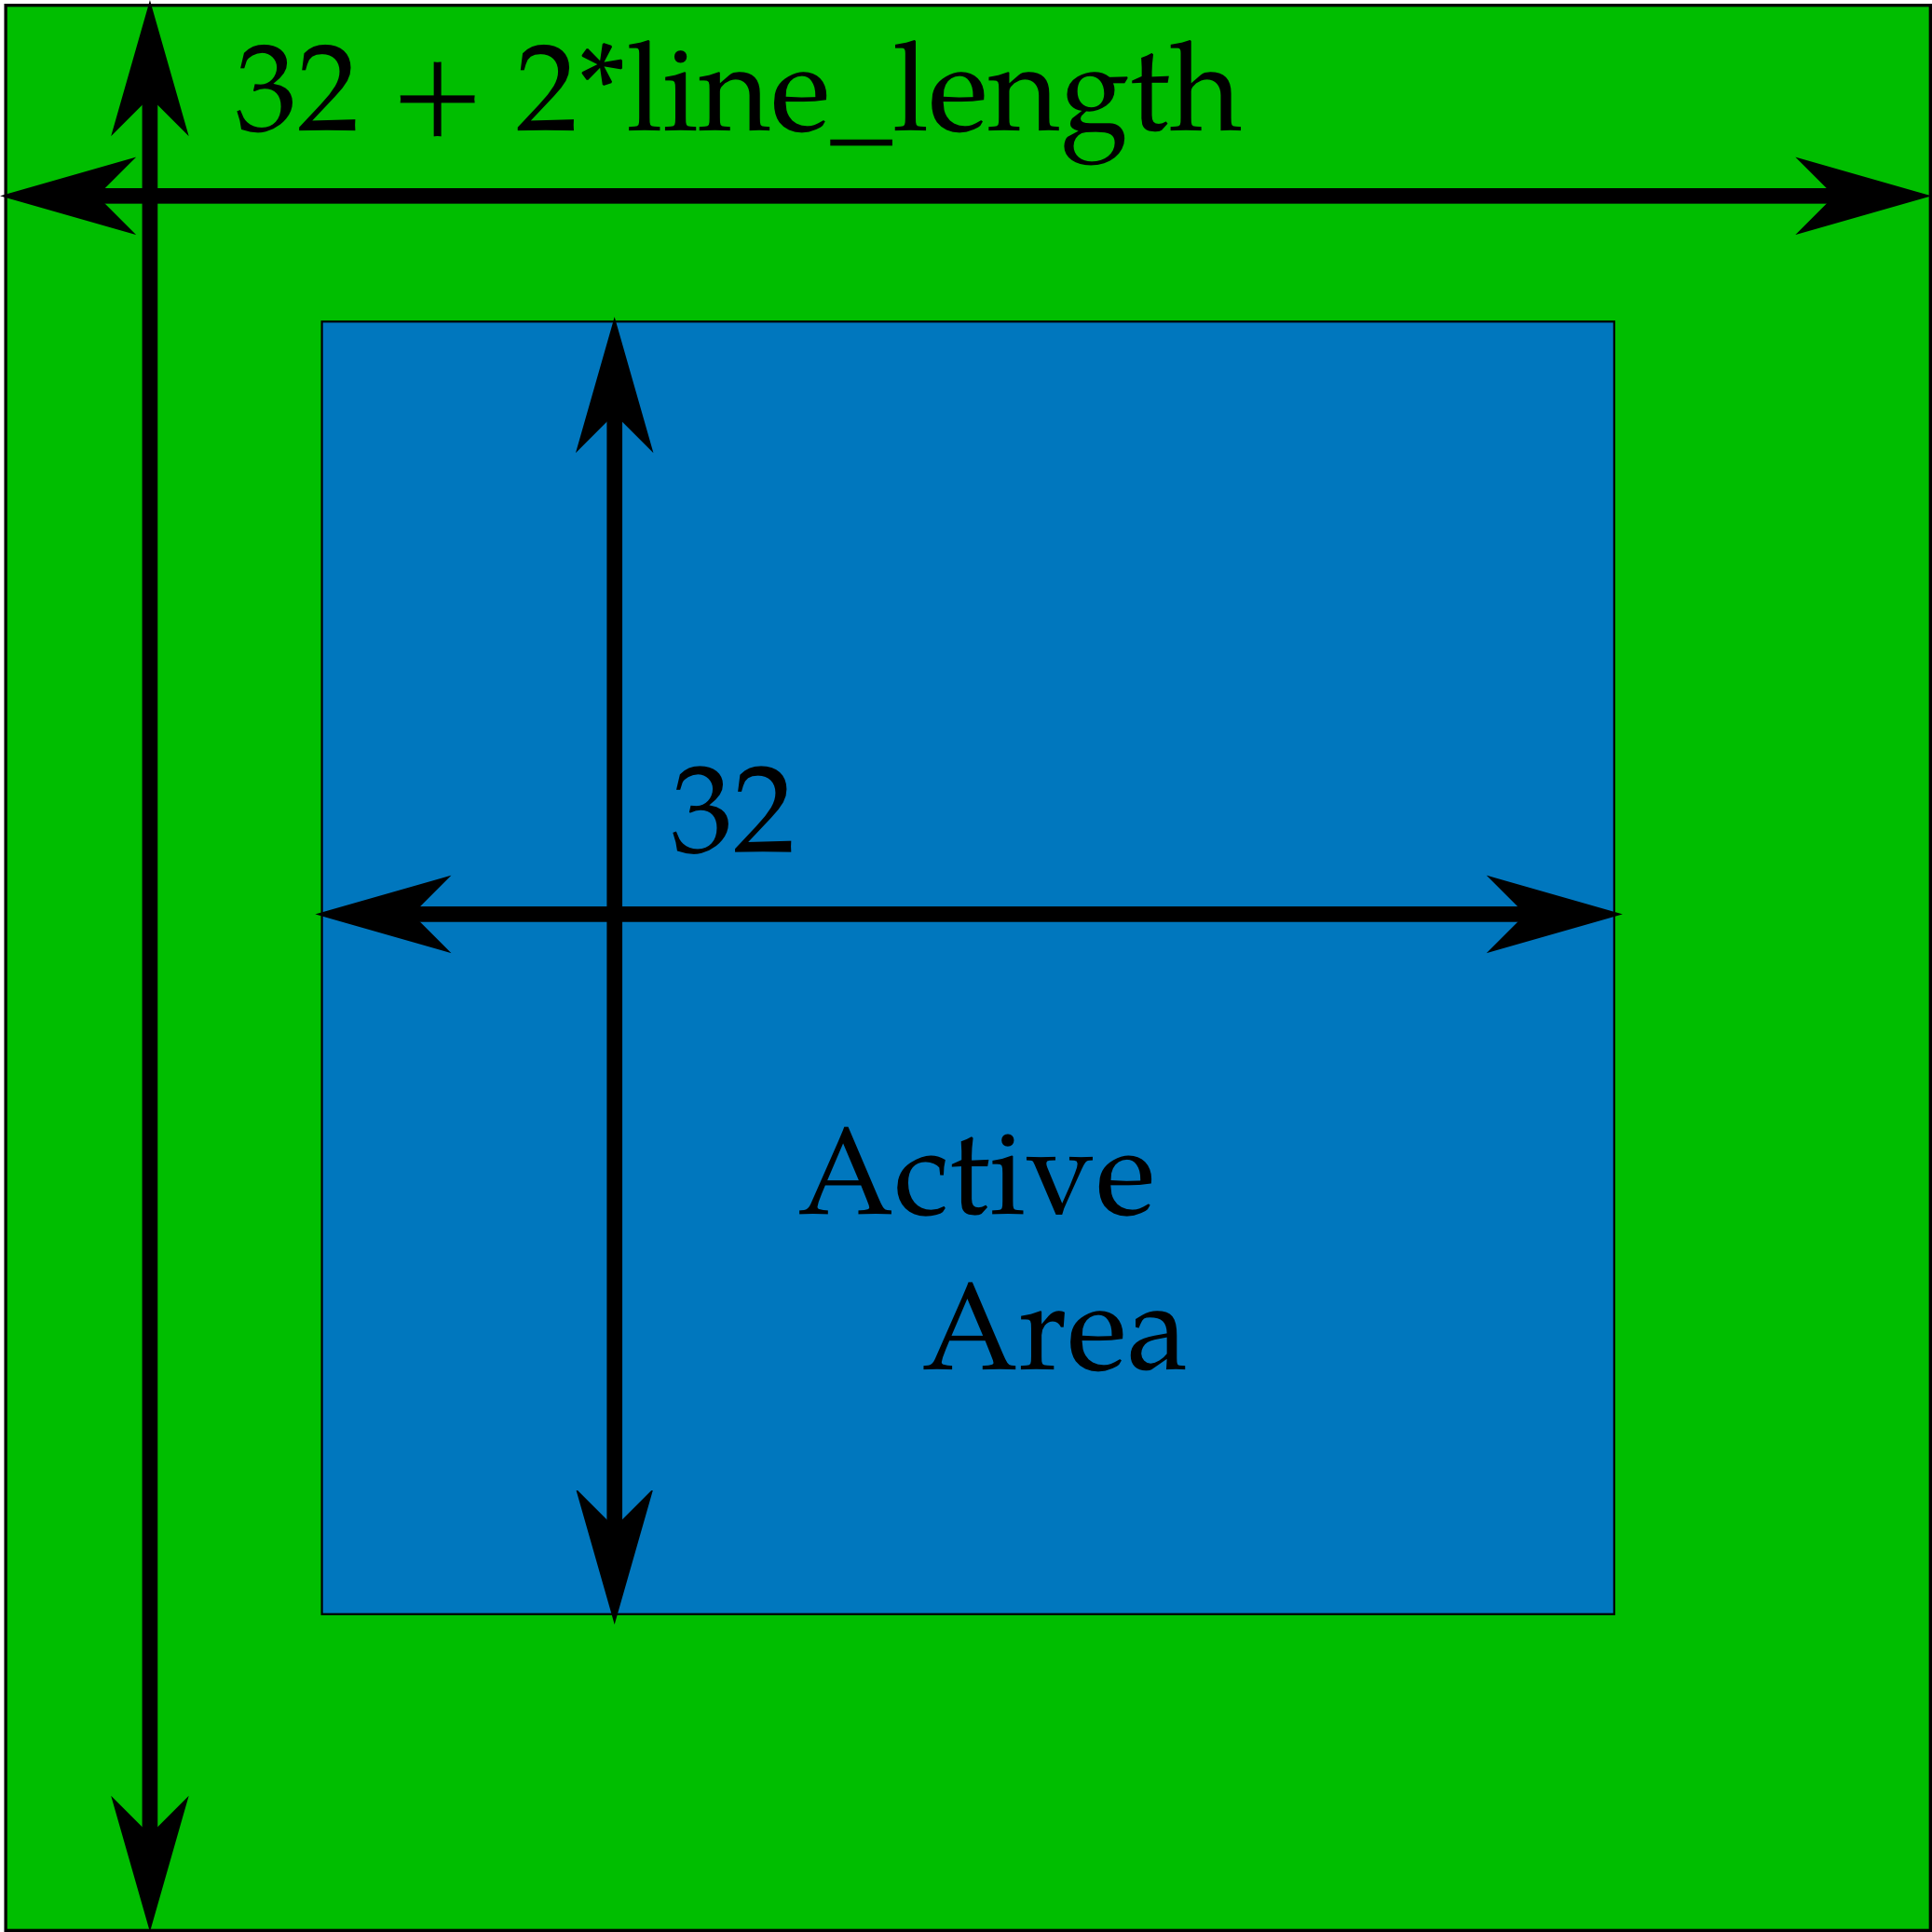
\includegraphics[width=0.2\textwidth]{images/shared-memory.png}
  \caption{Block and shared memory dimensions}
  \label{fig:shared-memory}
\end{figure}

On our device the maximum size of shared memory per block is $48kb$, so we can
only store a $109\times109$ block of float values. Therefore we only allow line
lengths up to 45 pixels.

The data from $G$ is copied by assigning the thread number to the linear
indexes of the data. As there is more data than threads, one thread copies
multiple data elements. The pattern is shown in \autoref{fig:shared-copy}.
\autoref{fig:shared-copy}.
\begin{figure}[htb]
  \centering
  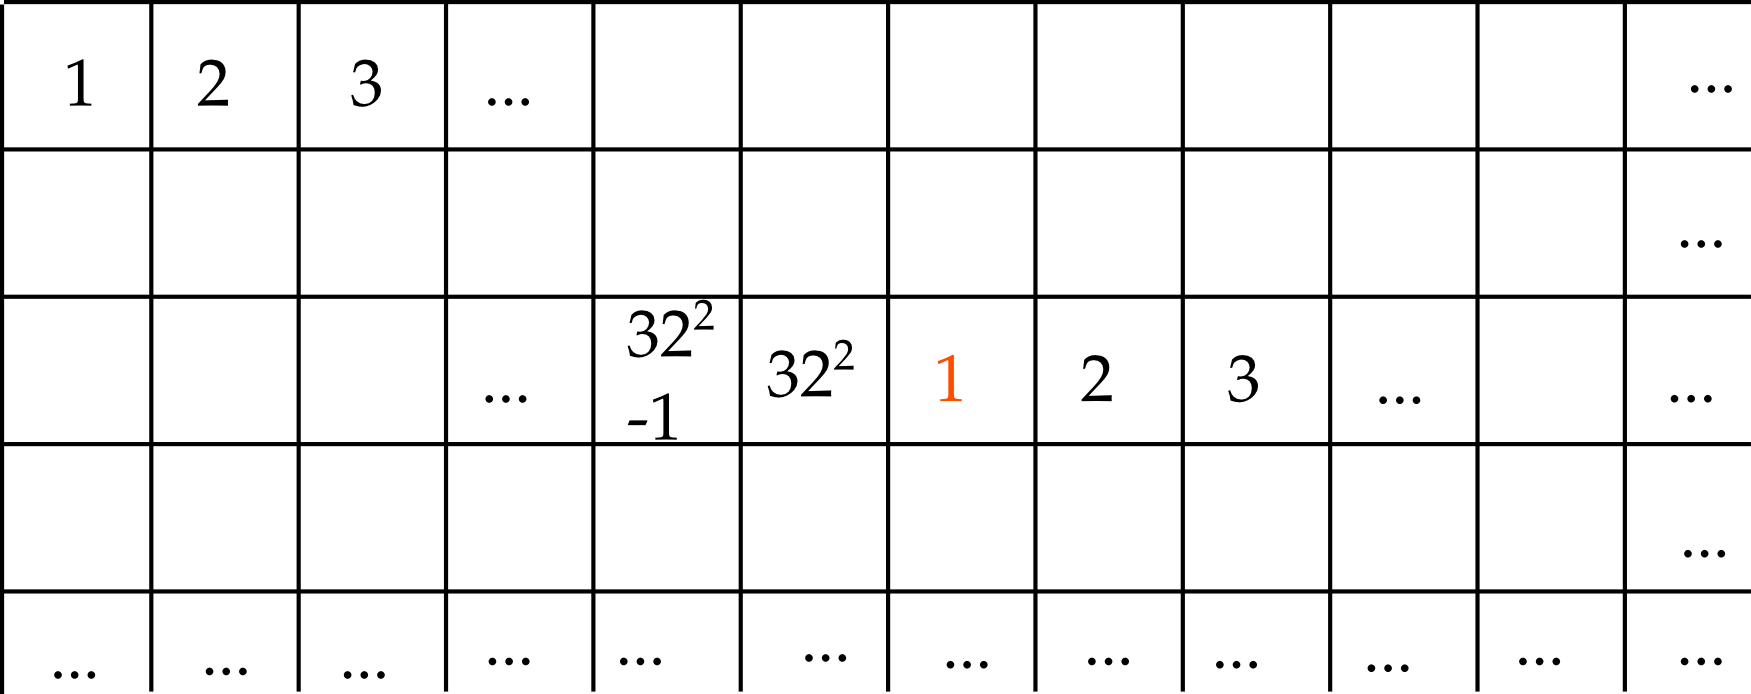
\includegraphics[width=0.5\textwidth]{images/shared-copy.png}
  \caption{Thread number assignment when copying the data from $G$ to shared memory.}
  \label{fig:shared-copy}
\end{figure}

The coordinate calculations for the line convolution computations are done such
that they generate the correct coordinates for the shared memory block. Due to
the coordinate rotations the access patterns are very chaotic, which might lead
to unavoidable bank conflicts.

Coordinates which lie outside the input image must not be included in the
copying process and later to calculate the convolution results.



\subsection{Histogram}
Andreeas

\subsection{Histogram Matching}
The histogram matching is used to adjust the tone distribution of the 
grayscale image to match a specific target tone distribution by using
their corresponding histogram. In this context, the target tone
distribution is artificially created to be similar to those of pencil
sketches as explained above.

The cumulative target histogram is created on the CPU by simply applying
the the parametric model to the values 0 to 255 and summing it up with
the values below.
This step is done on the CPU as the target distribution only has to
be evaluated 256 times which is negligible effort and can be either be
precomputed or done while the GPU is busy with other steps of the pipeline.

Once this histogram is uploaded to the GPU it can be used together with
the histogram from the image created in the previous step to adjust the
tones of the grayscale image. This is done in a kernel with one thread
per image pixel. A thread will the obtain the tone value of the pixel
it corresponds to and look up it's cumulative probability value in
the source histogram map.
Afterwards, the cumulative target histogram is used in inverse to find
out which tone the value corresponds to in it. The pixel is then set to
the looked up target tone value.

The inverse lookup in the cumulative target histogram is implemented
as a binary search function which is used in the kernel. Although
one would think that a binary search is inefficient when multiple threads
are executed in a warp and search for different values, it really isn't.
As the cumulative target histogram map only consist of 256 values,
the binary search will need at maximum $log_2 256=8$ loop runs to end
up at the correct value. Because the threads are executed in a warp,
the branches might get executed in serial. However, there is just one 
real branching operation inside the loop body, which could double the
effort. Still, the total effort negligible in contrast to a linear search
through the map with a worst case complexity of 256.

\subsection{Texturing}
Equation dings Raphael
